\chapter{Lecture 2 (01/19)}

This lecture was held on \textbf{January 19th, 2023}. It covered the equations of motion for damped and driven oscillators, as well as their applications in modern circuits.

\section{Last time: The Free Oscillator}

On Tuesday we explored oscillatory mechanics where there were no other forces besides the restoring force. However, in most systems, we will always have some kind of \textit{daming force} which impedes motion. This doesn't always have to be the case, but we will first explore a damping force which is proportional to the velocity: 

\[ \vec f = b \vec v\]

Under this, we now have the restoring force and the damping force, so Newton's second law now reads: 

\[ m \ddot x + b \dot x + kx = 0\] 

And so if we let $\beta = \frac{b}{2m}$ (we'll see later why this substitution is useful), then we can write

\[ \ddot x + 2\beta x + \omega_0^2 x = 0\]

The nature of these differential equations is that due to their linearity, if we find two independent solutions $x_1(t)$ and $x_2(t)$, then in general their solution will be a linear combination of the two: 

\[ x(t) = C_1x_1(t) + C_2x_2(t)\] 

We saw that exponentials worked before, let's have that as our main guess. Let 

\[ x(t) = e^{rt} \implies \dot x(t) = re^{rt}, \ddot x(t) = r^2e^{rt}\] 

Plugging this in, we get: 

\begin{align*}
    r^2e^{rt} + 2\beta r e^{rt} + \omega_0^2e^{rt} &= 0\\
    \therefore r^2 + 2\beta r + \omega_0^2 &= 0
\end{align*}

This is quadratic in $r$, so therefore we have solutions $r = -\beta \pm \sqrt{\beta^2 - \omega_0^2}$. Now, we can then write

\begin{align*}
    r_1 &= -\beta + \sqrt{\beta^2 - \omega_0^2}\\
    r_2 &= -\beta - \sqrt{\beta^2 - \omega_0^2}
\end{align*}

so the general solution now becomes: 

\[ x(t) = C_1e^{r_1t} + C_2e^{r_2t} = e^{-\beta t} \left( C_1e^{\sqrt{\beta^2 - \omega_0^2} t } + C_2e^{-\sqrt{\beta^2 - \omega_0^2}t}\right)\]

This equation makes sense intuitively, since a large value of $\beta$ generates a faster decay, which makes sense since $\beta$ refers to the damping constant. 

Now we have 3 cases that we want to analyze: 

\begin{enumerate}[label = (\alph*)]
    \item Underdamped: $\omega_0^2 > \beta^2$ 
    \item Critical damping: $\omega_0^2 = \beta^2$
    \item Overdamped: $\omega_0^2 < \beta^2$
\end{enumerate}

As it will turn out, only the overdamping will give us oscillatory motion.

\subsection{Case 1: Underdamped Oscillation} 

Here we look at the case where $\omega_0^2 > \beta^2$. If this is the case, then we can write $\sqrt{\beta^2 - \omega_0^2} = i\sqrt{\omega_0^2 - \beta^2} = i\omega_1$, with $\omega_1 = \sqrt{\omega_0^2 - \beta^2}$

\begin{insight*}{}{}
    if $\beta = 0$, then we exactly recover the solution that we got last time: 

    \[ x(t) = C_1e^{\sqrt{-\omega_0^2}t} + C_2e^{-\sqrt{-\omega_0^2}t} = C_1e^{i\omega_0t} + C_2e^{-i\omega_0t}\]

    This is a good way to check that what we're doing still makes sense.
\end{insight*}

There's also the case where we get \textit{weak underdamping}, where essentially we have $\beta \ll \omega_0$, so we get instead $x(t) = e^{-\beta t}\left(C_1e^{i\omega_1t} + C_2e^{-i\omega_1t}\right)$. Here, the $e^{-\beta t}$ term goes to zero over time, and the second term is just oscillation with $\omega_0 \to \omega_1$, so we can interpret this as an oscillation with an envelope of a decaying exponential. A diagram representation: 

\begin{center}
    \begin{tikzpicture}[samples=100, domain=0:5]

        \draw[->] (0, 0) -- (5.5,0) node[right] {$t$};
        \draw[->] (0,-2) -- (0,2) node[above] {$x(t)$};

        \draw[color=blue] plot (\x, {cos(5 * \x r) *exp(-0.5 * \x)}) node[above] {$x(t)$};
        \draw[color=red, dashed] plot (\x, {exp(-0.5 * \x)});
        \draw[color=red, dashed] plot (\x, {-exp(-0.5 * \x)});
        \node[color=red] at (3, 0.7) {$e^{-\beta t}$};
        \node[color=red] at (3, -0.7) {$-e^{-\beta t}$};
    \end{tikzpicture}
\end{center}

Here, the red dashed lines represent the envelope, and the $x(t)$ represents the actual motion. As we can see, the oscillation goes to zero over time, which makes sense since the damping force is constantly taking away energy. 

\subsection{Case 2: Damped Oscillation}

Now we look at $\omega_0^2 < \beta^2$. Here, the exponentials are real, so we can write:

\[ x(t) = C_1e^{-(\beta - \sqrt{\beta^2 - \omega_0^2})t} + C_2 e^{-(\beta + \sqrt{\beta^2 - \omega_0^2})t}\] 

On large time scales, we can see that the oscillation is dominated by the slower of the two exponentials (the faster one just dies out quicker, so we don't see it for large times). Interestingly, the rate of decay is lower if $\beta$ is larger, and we can see that since the exponentials get larger. 

When solving these problems, there are three cases we need to specifically look at if we let $x(0) = x_0 > 0$: 

\begin{itemize}
    \item $\dot{x_0} > 0$ such that we reach the maximum then the pendulum comes back.
    \item $\dot{x_0} < 0$ but we approach $x = 0$ but we do not go past. 
    \item Same as the previous case, but we do end up going past $x = 0$.
\end{itemize}

\subsection{Case 3: Critical Damping}

Now we look at $\omega_0^2 = \beta^2$, the most interesting case. Here, this means that the roots of $r^2 + 2\beta r + \omega_0^2 = 0$ are equal, so our solution becomes

\[ x(t) = e^{\beta t}\] 

Well we know that this differential equation has two solutions, and there is indeed a second solution, $x(t) = xe^{\beta t}$. We can check that it satisfies the differential equation by plugging it in (you can do this on your own time)

A critically damped oscillator will approach equilibrium the fastest. This has important design consequences $-$ in times where we want to reduce oscillation, critically damped systems are especially useful. Below is an illustration of this: 

\begin{center}
    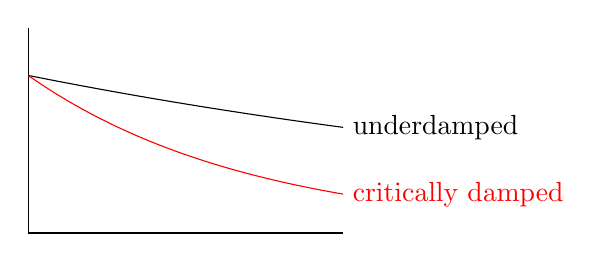
\begin{tikzpicture}[domain=0:2, samples=50, scale=2]
        \draw(0, 0) -- (2, 0);
        \draw(0, 0) -- (0, 1.3);
        \draw[color=black] plot (\x, {exp(-0.2* \x)}) node[right] {underdamped};
        \draw[color=red] plot (\x, {exp(-0.7 * \x)}) node[right] {critically damped};
    \end{tikzpicture}
\end{center}

Both of these curves are exponential decay curves, but the critically damped one goes to zero much faster than any other damping.

\section{Driving Forces}

Now imagine instead of a resistive force, that we have a driven force instead. That is, our equation of motion now looks like this: 

\[ F = -kx - bx + F_0 \cos(\omega t)\] 

where $F_0 \cos(\omega t)$ denotes the driving force, with $\omega$ being the angular frequency of the driving force. Therefore, we have the differential equation:

\[ \ddot x + 2\beta x + \omega_0^2x = f_0 \cos(\omega t)\] 

where $f_0 = \frac{F_0}{m}$, and $\beta$ is defin in the same way as before. This differential equation has two solutions: 

\begin{itemize}
    \item A homogeneous solution $x_h(t)$, which solves the differential equation when the right hand side is 0. 
    \item A particular soluiton, $x_p(t)$, which solves the differential equation while replicating the right hand side. 
\end{itemize}

Then, if we can find these two solutions, then we can combine them together: 

\[ x(t) = x_h(t) + x_p(t)\] 

We already know $x_h(t)$ from the earlier section, so if we can find an $x_p(t)$, then we have the full solution to the problem. We've seen before that sines and cosines seem to work well with oscillations, so why not try the solution $x_p(t) = A\cos(\omega t - \delta)$. Plugging this in, we get: 

\begin{align*}
    -A\omega^2 \cos(\omega t - \delta) - 2\beta A \omega \sin (\omega t - \delta) + \omega_0^2 A \cos(\omega t - \delta) = f_0 \cos \omega t\\
    f_0 \cos (\omega t) - A(\omega_0^2 - \omega^2)\cos(\omega t - \delta) + 2\beta A \cos(\omega t - \delta) = 0
\end{align*}

Now we use the trigonometric identities:

\begin{align*}
    \cos(\alpha - \beta) &= \cos \alpha \cos \beta + \sin \alpha \sin \beta\\
    \sin(\alpha - \beta) &= \sin \alpha \cos \beta - \cos \alpha \sin \beta
\end{align*}
    
Doing so we get the equation:


\[ \left \{ f_0 - A\left[ (\omega_0^2 - \omega^2)\cos \delta + 2\omega \beta \sin \delta \right]\right \} \cos (\omega t) -  \left \{A\left[ (\omega_0^2 - \omega^2)\sin \delta - 2\omega \beta \cos(\omega t)\right] \right \} \sin(\omega t) = 0\] 

Since $\sin(\omega t)$ and $\cos(\omega t)$ are linearly independent functions, this euqation is only satisfied when both terms are zero. From the first term, we get:

\begin{align*}
    \tan \delta &= \frac{2\omega \beta}{\omega_0^2 - \omega^2} \\
    \therefore \delta &= \tan^{-1}\left(\frac{2\omega \beta}{\omega_0^2 - \omega^2}\right)
\end{align*}

Therefore, 

\[ \sin \delta = \frac{2\omega \beta}{\sqrt{(\omega_0^2 - \omega^2)^2 + 4\omega^2 \beta^2}} \phantom{aaa} \cos \delta = \frac{\omega_0^2 - \omega^2}{\sqrt{(\omega_0^2 - \omega^2)^2 + 4\omega^2 \beta^2}}\]

From the cosine term, we get: 

\begin{align*}
    A &= \frac{f_0}{(\omega_0^2 - \omega^2)\cos \delta + 2\omega \beta \sin \delta}\\
    &= \frac{f_0}{\sqrt{(\omega_0^2 - \omega^2) + 4\omega^2 \beta^2}}
\end{align*}

so now we finally have the particular solution: 

\[ x_p(t) = A\cos(\omega t - \delta) = \frac{f_0 \cos (\omega t - \delta)}{\sqrt{(\omega_0^2 - \omega^2) + 4\omega^2 \beta^2}}\]

So our general solution, (again $x(t) = x_h(t) + x_p(t)$) is

\[ x(t) = C_1e^{r_1t} + C_2e^{r_2t} + A\cos(\omega t - \delta)\] 

Note that for large time, the $x_h(t)$ terms die out, but the $x_p(t)$ terms don't, and dominate for large time $t \gg \frac 1 \beta$. In other words: 

\[ x(t \gg \frac{1}{\beta}) = x_p(t)\] 

\subsection{The phase difference}

Earlier we said that $\delta$ represents the phase differene between the action and the resulting motion: 

\[ \delta = \tan^{-1}\left(\frac{2\omega \beta}{\omega_0^2 - \omega^2}\right)\] 

For a fixed $\omega_0$, as $\omega$ increases from 0, we get that the phase increases from $\delta = 0$ to $\delta = \pi/2$ at $\omega = \omega_0$ and $\delta \to \pi$ as $\omega \to \infty$.

\subsection{Amplitude} 

At large times, it's useful to look at the effect of $\omega$ on the amplitude by looking at $x_p(t)$. To find where $A$ is maximized, we simply take $\frac{dA}{d\omega} = 0$, giving us $\omega_2 = \sqrt{\omega_0^2 - 2\beta^2}$, so the resonance frequency is lowered as damping $\beta$ is increased. This makes sense intuitively, since the larger value of $\beta$ means that our oscillation decays much faster. 

\begin{insight*}{}{}
    Note that we don't get any resonance frequencies for $\beta^2 > \omega_0^2/2$, since that's when the square root becomes complex-valued.
\end{insight*}

[INSERT TIKZ HERE]

\section{Summary} 

In summary, so far we've looked at free, damped and driven oscillations: 
\begin{itemize}
    \item Free oscillations: $\omega_0 = \frac{k}{m}$
    \item Damped oscillations: $\omega_1 = \omega_0^2 - \beta^2$
    \item Driven oscillations: $\omega_2 = \omega_0 - 2\beta^2$
\end{itemize}

This set of relations gives us $\omega_0 > \omega_1 > \omega_2$. The maximum amplitude is given by 

\[ A_{max} = \frac{f_0}{\sqrt{4\omega^2\beta^2}} = \frac{f_0}{2\omega \beta}\]

This equation tells us that if we make $\beta$ smaller, then $A_{max}$ increases and also becomes taller and narrower. We define the \textit{full width half maximum} ($\text{FWHM} = 2\beta$ ) to quanitfy this value. 

\subsection{Aside: Quality Factor} 

We sometimes define a quality factor $Q$ as the ration of the resonance position $\omega_0$ to its width $2\beta$:

\[ Q = \frac{\omega_0}{2\beta}\] 

This means that large values of $Q$ correspond to narrow resonance, and small values correspond to a wide resonance. 

\section{Application: LC Circuits}

We've learned in electricity and magnetism (and also 5BL) that a simple LC circuit also behaves like an oscillator, since it follows the equation: 

\[ L \frac{dI}{dt} + \frac 1c \int I \ dt = 0\] 

or in terms of the charge $q$: 

\[ L \ddot q + \frac{1}{c} q = 0\] 

The solutions are of the same form since the only thing we've changed here are the variable names: $q(t) = q_0 \cos(\omega t)$. Overall, we can just perform the substtution of letters: 

\[ m \to L \phantom{aa} x \to q \phantom{aa} \frac 1k \to c \phantom{aa} \dot x \to I\] 

Similarly, adding a resistance will give us the equivalent of a damping term, and adding an AC power generator is the same as adding a driving force to the system. Again, the nature of these system is the exact same as what we just solved for, so the equations of motion remain the same as well.




